% Options for packages loaded elsewhere
\PassOptionsToPackage{unicode}{hyperref}
\PassOptionsToPackage{hyphens}{url}
%
\documentclass[
]{article}
\usepackage{amsmath,amssymb}
\usepackage{lmodern}
\usepackage{ifxetex,ifluatex}
\ifnum 0\ifxetex 1\fi\ifluatex 1\fi=0 % if pdftex
  \usepackage[T1]{fontenc}
  \usepackage[utf8]{inputenc}
  \usepackage{textcomp} % provide euro and other symbols
\else % if luatex or xetex
  \usepackage{unicode-math}
  \defaultfontfeatures{Scale=MatchLowercase}
  \defaultfontfeatures[\rmfamily]{Ligatures=TeX,Scale=1}
\fi
% Use upquote if available, for straight quotes in verbatim environments
\IfFileExists{upquote.sty}{\usepackage{upquote}}{}
\IfFileExists{microtype.sty}{% use microtype if available
  \usepackage[]{microtype}
  \UseMicrotypeSet[protrusion]{basicmath} % disable protrusion for tt fonts
}{}
\makeatletter
\@ifundefined{KOMAClassName}{% if non-KOMA class
  \IfFileExists{parskip.sty}{%
    \usepackage{parskip}
  }{% else
    \setlength{\parindent}{0pt}
    \setlength{\parskip}{6pt plus 2pt minus 1pt}}
}{% if KOMA class
  \KOMAoptions{parskip=half}}
\makeatother
\usepackage{xcolor}
\IfFileExists{xurl.sty}{\usepackage{xurl}}{} % add URL line breaks if available
\IfFileExists{bookmark.sty}{\usepackage{bookmark}}{\usepackage{hyperref}}
\hypersetup{
  pdftitle={Final Project: Regression From The Mean},
  pdfauthor={Zhengtao Xu, Jennings Cheng and Collin Carmichael},
  hidelinks,
  pdfcreator={LaTeX via pandoc}}
\urlstyle{same} % disable monospaced font for URLs
\usepackage[margin=1in]{geometry}
\usepackage{color}
\usepackage{fancyvrb}
\newcommand{\VerbBar}{|}
\newcommand{\VERB}{\Verb[commandchars=\\\{\}]}
\DefineVerbatimEnvironment{Highlighting}{Verbatim}{commandchars=\\\{\}}
% Add ',fontsize=\small' for more characters per line
\usepackage{framed}
\definecolor{shadecolor}{RGB}{248,248,248}
\newenvironment{Shaded}{\begin{snugshade}}{\end{snugshade}}
\newcommand{\AlertTok}[1]{\textcolor[rgb]{0.94,0.16,0.16}{#1}}
\newcommand{\AnnotationTok}[1]{\textcolor[rgb]{0.56,0.35,0.01}{\textbf{\textit{#1}}}}
\newcommand{\AttributeTok}[1]{\textcolor[rgb]{0.77,0.63,0.00}{#1}}
\newcommand{\BaseNTok}[1]{\textcolor[rgb]{0.00,0.00,0.81}{#1}}
\newcommand{\BuiltInTok}[1]{#1}
\newcommand{\CharTok}[1]{\textcolor[rgb]{0.31,0.60,0.02}{#1}}
\newcommand{\CommentTok}[1]{\textcolor[rgb]{0.56,0.35,0.01}{\textit{#1}}}
\newcommand{\CommentVarTok}[1]{\textcolor[rgb]{0.56,0.35,0.01}{\textbf{\textit{#1}}}}
\newcommand{\ConstantTok}[1]{\textcolor[rgb]{0.00,0.00,0.00}{#1}}
\newcommand{\ControlFlowTok}[1]{\textcolor[rgb]{0.13,0.29,0.53}{\textbf{#1}}}
\newcommand{\DataTypeTok}[1]{\textcolor[rgb]{0.13,0.29,0.53}{#1}}
\newcommand{\DecValTok}[1]{\textcolor[rgb]{0.00,0.00,0.81}{#1}}
\newcommand{\DocumentationTok}[1]{\textcolor[rgb]{0.56,0.35,0.01}{\textbf{\textit{#1}}}}
\newcommand{\ErrorTok}[1]{\textcolor[rgb]{0.64,0.00,0.00}{\textbf{#1}}}
\newcommand{\ExtensionTok}[1]{#1}
\newcommand{\FloatTok}[1]{\textcolor[rgb]{0.00,0.00,0.81}{#1}}
\newcommand{\FunctionTok}[1]{\textcolor[rgb]{0.00,0.00,0.00}{#1}}
\newcommand{\ImportTok}[1]{#1}
\newcommand{\InformationTok}[1]{\textcolor[rgb]{0.56,0.35,0.01}{\textbf{\textit{#1}}}}
\newcommand{\KeywordTok}[1]{\textcolor[rgb]{0.13,0.29,0.53}{\textbf{#1}}}
\newcommand{\NormalTok}[1]{#1}
\newcommand{\OperatorTok}[1]{\textcolor[rgb]{0.81,0.36,0.00}{\textbf{#1}}}
\newcommand{\OtherTok}[1]{\textcolor[rgb]{0.56,0.35,0.01}{#1}}
\newcommand{\PreprocessorTok}[1]{\textcolor[rgb]{0.56,0.35,0.01}{\textit{#1}}}
\newcommand{\RegionMarkerTok}[1]{#1}
\newcommand{\SpecialCharTok}[1]{\textcolor[rgb]{0.00,0.00,0.00}{#1}}
\newcommand{\SpecialStringTok}[1]{\textcolor[rgb]{0.31,0.60,0.02}{#1}}
\newcommand{\StringTok}[1]{\textcolor[rgb]{0.31,0.60,0.02}{#1}}
\newcommand{\VariableTok}[1]{\textcolor[rgb]{0.00,0.00,0.00}{#1}}
\newcommand{\VerbatimStringTok}[1]{\textcolor[rgb]{0.31,0.60,0.02}{#1}}
\newcommand{\WarningTok}[1]{\textcolor[rgb]{0.56,0.35,0.01}{\textbf{\textit{#1}}}}
\usepackage{graphicx}
\makeatletter
\def\maxwidth{\ifdim\Gin@nat@width>\linewidth\linewidth\else\Gin@nat@width\fi}
\def\maxheight{\ifdim\Gin@nat@height>\textheight\textheight\else\Gin@nat@height\fi}
\makeatother
% Scale images if necessary, so that they will not overflow the page
% margins by default, and it is still possible to overwrite the defaults
% using explicit options in \includegraphics[width, height, ...]{}
\setkeys{Gin}{width=\maxwidth,height=\maxheight,keepaspectratio}
% Set default figure placement to htbp
\makeatletter
\def\fps@figure{htbp}
\makeatother
\setlength{\emergencystretch}{3em} % prevent overfull lines
\providecommand{\tightlist}{%
  \setlength{\itemsep}{0pt}\setlength{\parskip}{0pt}}
\setcounter{secnumdepth}{-\maxdimen} % remove section numbering
\ifluatex
  \usepackage{selnolig}  % disable illegal ligatures
\fi

\title{Final Project: Regression From The Mean}
\author{Zhengtao Xu, Jennings Cheng and Collin Carmichael}
\date{8/6/2021}

\begin{document}
\maketitle

\textbf{Section 1: Introduction}

\textbf{Section 2: Exploratory Data Analysis}

\includegraphics{Final_Project_2_files/figure-latex/unnamed-chunk-3-1.pdf}
Looking at a correlation heatmap we see aside from dewpoint
precipitation and temperature there are no significant correlation in
other variable

\includegraphics{Final_Project_2_files/figure-latex/unnamed-chunk-4-1.pdf}
We can see that PM2.5 has an inverse distribution with values skewed
towards low PM2.5 but many high values that go beyond the median

Temp and Dew point are highly related and so may not need to be included
in the same model

Precipitation looks like a bell curve but not normal as seen in the plot
in 3,3

Wind speed is similar but not identical to PM2.5 in that it has an
inverse distribution so it may be highly important in prediction

There is almost always not any snow in Beijing and the max is 27 for a
day

Rain is also infrequent but there are times when there is a lot of rain
so we may assume that rain and snow are not the same

The most common direction is SE and NW while sometimes NE or CV

Now that we know the distributions we can take a look at some pm2.5 vs
predictor

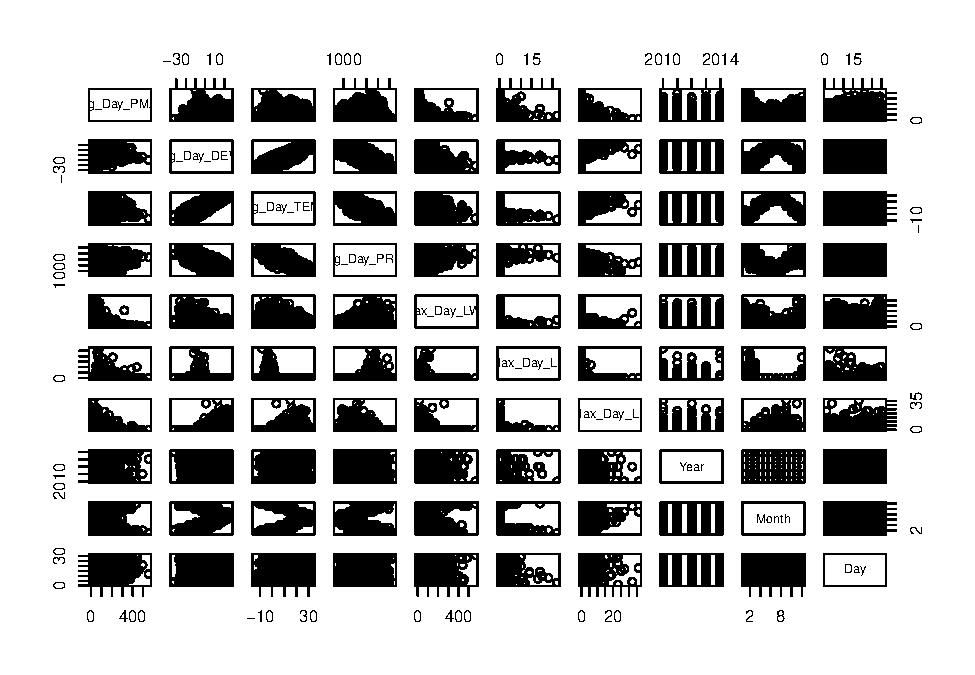
\includegraphics[width=0.9\linewidth,height=0.75\textheight]{Final_Project_2_files/figure-latex/unnamed-chunk-5-1}

we can see pm2.5 against time is not a clear relationship and there are
many seasonal spikes - One thing is that since there are random
fluctations in our final model we will not use date since in a
regression model the advance of one day would theoretically advance
pm2.5 which is not the relationship we see

We can also extract that dew, temp, pres are very clearly related from
the following:

\includegraphics[width=0.8\linewidth,height=0.8\textheight]{Final_Project_2_files/figure-latex/unnamed-chunk-6-1}
Dew and temp are very similar and pres is the opposite so we may not
necessarily need all three in the final model

Max wind is also related to Avg\_Day\_PM2.5 since more wind produces
less 2.5

At first glance it may seem that pm2.5 may not vary with month day or
year since there are a lot of random spike but looking at a mean of all
pm2.5 with each factor shows us that it indeed is influenced highly by
these predictor
\includegraphics{Final_Project_2_files/figure-latex/unnamed-chunk-7-1.pdf}
As we see the variation between the month year and day is important and
vary so therefore for the sake of fitting a model between these years
every variable will be important beside Date\_D

\textbf{3.1: Fitting model and diagnostic}

\begin{verbatim}
## 
## Call:
## lm(formula = Avg_Day_PM2.5 ~ ., data = trainingdate)
## 
## Residuals:
##     Min      1Q  Median      3Q     Max 
## -160.66  -41.35  -10.03   29.74  319.93 
## 
## Coefficients:
##                  Estimate Std. Error t value Pr(>|t|)    
## (Intercept)    -1.140e+03  2.355e+03  -0.484 0.628449    
## Avg_Day_DEWP    6.982e+00  3.505e-01  19.919  < 2e-16 ***
## Avg_Day_TEMP   -1.044e+01  4.421e-01 -23.607  < 2e-16 ***
## Avg_Day_PRES   -2.553e+00  3.318e-01  -7.694 2.64e-14 ***
## Max_Day_LWS    -1.635e-01  2.733e-02  -5.984 2.76e-09 ***
## Max_Day_LS     -4.152e+00  1.017e+00  -4.084 4.68e-05 ***
## Max_Day_LR     -5.222e+00  6.323e-01  -8.258 3.34e-16 ***
## Max_Day_CBWDNE -8.079e+01  1.804e+01  -4.477 8.17e-06 ***
## Max_Day_CBWDNW -5.723e+01  1.678e+01  -3.410 0.000669 ***
## Max_Day_CBWDSE -5.064e+01  1.673e+01  -3.028 0.002510 ** 
## Year            1.999e+00  1.167e+00   1.713 0.086910 .  
## Month          -1.859e+00  5.206e-01  -3.570 0.000369 ***
## Day             7.338e-01  1.847e-01   3.972 7.49e-05 ***
## ---
## Signif. codes:  0 '***' 0.001 '**' 0.01 '*' 0.05 '.' 0.1 ' ' 1
## 
## Residual standard error: 61.27 on 1421 degrees of freedom
##   (26 observations deleted due to missingness)
## Multiple R-squared:  0.4042, Adjusted R-squared:  0.3991 
## F-statistic: 80.33 on 12 and 1421 DF,  p-value: < 2.2e-16
\end{verbatim}

\includegraphics{Final_Project_2_files/figure-latex/unnamed-chunk-8-1.pdf}

\begin{verbatim}
##    (Intercept)   Avg_Day_DEWP   Avg_Day_TEMP   Avg_Day_PRES    Max_Day_LWS 
##   6.284491e-01   4.717073e-78  3.203974e-104   2.643099e-14   2.759269e-09 
##     Max_Day_LS     Max_Day_LR Max_Day_CBWDNE Max_Day_CBWDNW Max_Day_CBWDSE 
##   4.680786e-05   3.341618e-16   8.172423e-06   6.685417e-04   2.509930e-03 
##           Year          Month            Day 
##   8.690987e-02   3.685244e-04   7.488178e-05
\end{verbatim}

\begin{verbatim}
## $r.squared
## [1] 0.4041776
\end{verbatim}

After fitting a full model we see every single predictor besides year is
significant however R square is only 0.4 which suggests even though each
coefficient is directionally correct the variation of response is not
accurate

We can see some diagnostics as to why our model may not be that
effective

\begin{Shaded}
\begin{Highlighting}[]
\CommentTok{\#partialregress}


\NormalTok{r.ydew}\OtherTok{=}\FunctionTok{update}\NormalTok{(lm\_all , }\SpecialCharTok{\textasciitilde{}}\NormalTok{. }\SpecialCharTok{{-}}\NormalTok{ Avg\_Day\_DEWP)}\SpecialCharTok{$}\NormalTok{res}
\NormalTok{nonatrain }\OtherTok{\textless{}{-}} \FunctionTok{na.omit}\NormalTok{(trainingdate)}
\NormalTok{r.dew}\OtherTok{=}\FunctionTok{lm}\NormalTok{(Avg\_Day\_DEWP }\SpecialCharTok{\textasciitilde{}}\NormalTok{ . , }\AttributeTok{data =}\NormalTok{ nonatrain[ , }\SpecialCharTok{{-}} \DecValTok{1}\NormalTok{ ])}\SpecialCharTok{$}\NormalTok{res}
\NormalTok{tmp}\OtherTok{=}\FunctionTok{lm}\NormalTok{(r.ydew }\SpecialCharTok{\textasciitilde{}}\NormalTok{ r.dew )}

\NormalTok{tmp}
\end{Highlighting}
\end{Shaded}

\begin{verbatim}
## 
## Call:
## lm(formula = r.ydew ~ r.dew)
## 
## Coefficients:
## (Intercept)        r.dew  
##   6.147e-15    6.982e+00
\end{verbatim}

\begin{Shaded}
\begin{Highlighting}[]
\NormalTok{r.ytemp}\OtherTok{=}\FunctionTok{update}\NormalTok{(lm\_all , }\SpecialCharTok{\textasciitilde{}}\NormalTok{. }\SpecialCharTok{{-}}\NormalTok{Avg\_Day\_TEMP)}\SpecialCharTok{$}\NormalTok{res}
\NormalTok{r.temp}\OtherTok{=}\FunctionTok{lm}\NormalTok{(Avg\_Day\_TEMP }\SpecialCharTok{\textasciitilde{}}\NormalTok{ . , }\AttributeTok{data =}\NormalTok{ nonatrain [ , }\SpecialCharTok{{-}}\DecValTok{1}\NormalTok{ ])}\SpecialCharTok{$}\NormalTok{res}
\NormalTok{tmptemp}\OtherTok{=}\FunctionTok{lm}\NormalTok{(r.ytemp}\SpecialCharTok{\textasciitilde{}}\NormalTok{r.temp)}
\NormalTok{r.ypres}\OtherTok{=}\FunctionTok{update}\NormalTok{(lm\_all ,}\SpecialCharTok{\textasciitilde{}}\NormalTok{. }\SpecialCharTok{{-}}\NormalTok{ Avg\_Day\_PRES)}\SpecialCharTok{$}\NormalTok{res}
\NormalTok{r.pres}\OtherTok{=}\FunctionTok{lm}\NormalTok{(Avg\_Day\_PRES }\SpecialCharTok{\textasciitilde{}}\NormalTok{. , }\AttributeTok{data=}\NormalTok{nonatrain[,}\SpecialCharTok{{-}}\DecValTok{1}\NormalTok{])}\SpecialCharTok{$}\NormalTok{res}
\NormalTok{tmppres}\OtherTok{=}\FunctionTok{lm}\NormalTok{(r.ypres}\SpecialCharTok{\textasciitilde{}}\NormalTok{r.pres)}
\NormalTok{r.ylws}\OtherTok{=}\FunctionTok{update}\NormalTok{(lm\_all,}\SpecialCharTok{\textasciitilde{}}\NormalTok{. }\SpecialCharTok{{-}}\NormalTok{Max\_Day\_WLS)}\SpecialCharTok{$}\NormalTok{res}
\NormalTok{r.lws}\OtherTok{=}\FunctionTok{lm}\NormalTok{(Max\_Day\_LWS }\SpecialCharTok{\textasciitilde{}}\NormalTok{.,}\AttributeTok{data=}\NormalTok{nonatrain[,}\SpecialCharTok{{-}}\DecValTok{1}\NormalTok{])}\SpecialCharTok{$}\NormalTok{res}
\NormalTok{tmplws}\OtherTok{=}\FunctionTok{lm}\NormalTok{(r.ylws}\SpecialCharTok{\textasciitilde{}}\NormalTok{r.lws)}
\NormalTok{r.yls }\OtherTok{\textless{}{-}} \FunctionTok{update}\NormalTok{(lm\_all,}\SpecialCharTok{\textasciitilde{}}\NormalTok{. }\SpecialCharTok{{-}}\NormalTok{Max\_Day\_LS)}\SpecialCharTok{$}\NormalTok{res}
\NormalTok{r.ls }\OtherTok{\textless{}{-}} \FunctionTok{lm}\NormalTok{( Max\_Day\_LS }\SpecialCharTok{\textasciitilde{}}\NormalTok{. , }\AttributeTok{data=}\NormalTok{ nonatrain [ ,}\SpecialCharTok{{-}}\DecValTok{1}\NormalTok{ ])}\SpecialCharTok{$}\NormalTok{res}
\NormalTok{tmpls }\OtherTok{\textless{}{-}} \FunctionTok{lm}\NormalTok{(r.yls}\SpecialCharTok{\textasciitilde{}}\NormalTok{r.ls)}
\NormalTok{r.ylr }\OtherTok{\textless{}{-}} \FunctionTok{update}\NormalTok{(lm\_all ,}\SpecialCharTok{\textasciitilde{}}\NormalTok{. }\SpecialCharTok{{-}}\NormalTok{ Max\_Day\_LR)}\SpecialCharTok{$}\NormalTok{res}
\NormalTok{r.lr }\OtherTok{\textless{}{-}} \FunctionTok{lm}\NormalTok{(Max\_Day\_LR }\SpecialCharTok{\textasciitilde{}}\NormalTok{.,}\AttributeTok{data =}\NormalTok{ nonatrain[ , }\SpecialCharTok{{-}}\DecValTok{1}\NormalTok{ ] )}\SpecialCharTok{$}\NormalTok{res}
\NormalTok{tmplr }\OtherTok{\textless{}{-}} \FunctionTok{lm}\NormalTok{(r.ylr }\SpecialCharTok{\textasciitilde{}}\NormalTok{ r.lr )}
\NormalTok{r.yyear }\OtherTok{=} \FunctionTok{update}\NormalTok{ (lm\_all,}\SpecialCharTok{\textasciitilde{}}\NormalTok{.}\SpecialCharTok{{-}}\NormalTok{Year)}\SpecialCharTok{$}\NormalTok{res}
\NormalTok{r.year}\OtherTok{=}\FunctionTok{lm}\NormalTok{(Year}\SpecialCharTok{\textasciitilde{}}\NormalTok{.,}\AttributeTok{data=}\NormalTok{nonatrain[ , }\SpecialCharTok{{-}}\DecValTok{1}\NormalTok{ ] )}\SpecialCharTok{$}\NormalTok{res}
\NormalTok{tmpyear}\OtherTok{=}\FunctionTok{lm}\NormalTok{(r.yyear}\SpecialCharTok{\textasciitilde{}}\NormalTok{r.year)}
\NormalTok{r.ymonth }\OtherTok{=} \FunctionTok{update}\NormalTok{ (lm\_all,}\SpecialCharTok{\textasciitilde{}}\NormalTok{.}\SpecialCharTok{{-}}\NormalTok{Month)}\SpecialCharTok{$}\NormalTok{res}
\NormalTok{r.month }\OtherTok{=} \FunctionTok{lm}\NormalTok{(Month}\SpecialCharTok{\textasciitilde{}}\NormalTok{.,}\AttributeTok{data=}\NormalTok{nonatrain[,}\SpecialCharTok{{-}}\DecValTok{1}\NormalTok{])}\SpecialCharTok{$}\NormalTok{res}
\NormalTok{tmpmonth}\OtherTok{=}\FunctionTok{lm}\NormalTok{(r.ymonth}\SpecialCharTok{\textasciitilde{}}\NormalTok{r.month)}
\NormalTok{r.yday}\OtherTok{=}\FunctionTok{update}\NormalTok{(lm\_all,}\SpecialCharTok{\textasciitilde{}}\NormalTok{.}\SpecialCharTok{{-}}\NormalTok{Day)}\SpecialCharTok{$}\NormalTok{res}
\NormalTok{r.day}\OtherTok{=}\FunctionTok{lm}\NormalTok{(Day}\SpecialCharTok{\textasciitilde{}}\NormalTok{.,}\AttributeTok{data=}\NormalTok{nonatrain[,}\SpecialCharTok{{-}}\DecValTok{1}\NormalTok{])}\SpecialCharTok{$}\NormalTok{res}
\NormalTok{tmpday}\OtherTok{=}\FunctionTok{lm}\NormalTok{(r.yday}\SpecialCharTok{\textasciitilde{}}\NormalTok{r.day)}
\CommentTok{\#5x2 to show each}
\NormalTok{titles}\OtherTok{=}\StringTok{\textquotesingle{}pollution daily res\textquotesingle{}}
\FunctionTok{par}\NormalTok{(}\AttributeTok{mfrow=}\FunctionTok{c}\NormalTok{(}\DecValTok{2}\NormalTok{,}\DecValTok{5}\NormalTok{))}
\FunctionTok{plot}\NormalTok{(r.dew,r.ydew,}\AttributeTok{xlab=}\StringTok{"dew residual"}\NormalTok{,}\AttributeTok{ylab=}\NormalTok{titles)}
\FunctionTok{abline}\NormalTok{(tmp)}


\FunctionTok{plot}\NormalTok{(r.temp,r.ytemp,}\AttributeTok{xlab=}\StringTok{"temp residual"}\NormalTok{,}\AttributeTok{ylab=}\NormalTok{titles)}
\FunctionTok{abline}\NormalTok{(tmptemp)}
\FunctionTok{plot}\NormalTok{(r.pres,r.ypres,}\AttributeTok{xlab=}\StringTok{"pres residual"}\NormalTok{,}\AttributeTok{ylab=}\NormalTok{ titles)}
\FunctionTok{abline}\NormalTok{(tmppres)}

\FunctionTok{plot}\NormalTok{(r.lws,r.ylws,}\AttributeTok{xlab=}\StringTok{"lws residual"}\NormalTok{,}\AttributeTok{ylab=}\NormalTok{titles)}
\FunctionTok{abline}\NormalTok{(tmplws)}
\FunctionTok{plot}\NormalTok{(r.ls,r.yls,}\AttributeTok{xlab=}\StringTok{\textquotesingle{}ls residual\textquotesingle{}}\NormalTok{,}\AttributeTok{ylab=}\NormalTok{titles)}
\FunctionTok{abline}\NormalTok{(tmpls)}
\FunctionTok{plot}\NormalTok{(r.lr,r.ylr,}\AttributeTok{xlab=}\StringTok{\textquotesingle{}lr residual\textquotesingle{}}\NormalTok{,}\AttributeTok{ylab=}\NormalTok{titles)}
\FunctionTok{abline}\NormalTok{(tmplr)}
\FunctionTok{plot}\NormalTok{(r.year,r.yyear,}\AttributeTok{xlab=}\StringTok{\textquotesingle{}year residual\textquotesingle{}}\NormalTok{ , }\AttributeTok{ylab=}\NormalTok{titles)}
\FunctionTok{abline}\NormalTok{(tmpyear)}

\FunctionTok{plot}\NormalTok{(r.month,r.ymonth,}\AttributeTok{xlab=}\StringTok{"month residual"}\NormalTok{,}\AttributeTok{ylab=}\NormalTok{titles)}
\FunctionTok{abline}\NormalTok{(tmpmonth)}
\FunctionTok{plot}\NormalTok{(r.day,r.yday,}\AttributeTok{xlab=}\StringTok{"day residual"}\NormalTok{,}\AttributeTok{ylab=}\NormalTok{titles)}
\FunctionTok{abline}\NormalTok{(tmpday)}
\end{Highlighting}
\end{Shaded}

\includegraphics{Final_Project_2_files/figure-latex/unnamed-chunk-9-1.pdf}
We see that there are a lot of high influence points in partial
regression for each numerical variable

Now we can check some of the plot of diagnostic

\includegraphics{Final_Project_2_files/figure-latex/unnamed-chunk-12-1.pdf}
Taking a glance at our linear model, we see that it does not appear to
meet all error assumptions. Particularly, the Q-Q plot suggests
non-normality and the Fitted-Residual plot suggests heteroscedasticity
and some degree of non-linearity. However, the Residuals-Leverage plot
appears to indicate that we don't have any high influence points.

\begin{verbatim}
## 
##  studentized Breusch-Pagan test
## 
## data:  lm_all
## BP = 175.74, df = 12, p-value < 2.2e-16
\end{verbatim}

\begin{verbatim}
## 
##  Shapiro-Wilk normality test
## 
## data:  residuals(lm_all)
## W = 0.93117, p-value < 2.2e-16
\end{verbatim}

\begin{verbatim}
## 
##  Durbin-Watson test
## 
## data:  lm_all
## DW = 1.0114, p-value < 2.2e-16
## alternative hypothesis: true autocorrelation is greater than 0
\end{verbatim}

\includegraphics{Final_Project_2_files/figure-latex/unnamed-chunk-13-1.pdf}
As we can tell through testing more formally, none of the error
assumptions of homocedasticity, normality, and uncorrelated errors are
accurate.

\includegraphics{Final_Project_2_files/figure-latex/unnamed-chunk-14-1.pdf}
In regards to unusual observations, our maximum cooks distance as seen
above indicates we have no datapoints that would be classified as highly
influential, since it is much less than one. In constrast, however, we
seem to have an abundance of high-leverage points. However, it is
unclear at first glance how many of these are ``good'' or ``bad''
leverage points, although we can assume some points like observations 3
and 1468 with wildly different y-values are likely ``bad.''

\begin{verbatim}
##             b d        c
## 417  4.327428 > 4.152348
## 1108 5.299076 > 4.152348
## 1477 4.762509 > 4.152348
## 1517 4.561424 > 4.152348
\end{verbatim}

As we can see above, we also have four outliers in the dataset.

So in order to remedy non linearity, heteroscedasticity, non normal
residual and autocorrelation we would try to

\includegraphics{Final_Project_2_files/figure-latex/unnamed-chunk-16-1.pdf}

\begin{verbatim}
##             b d        c
## 417  4.327428 > 4.152348
## 1108 5.299076 > 4.152348
## 1477 4.762509 > 4.152348
## 1517 4.561424 > 4.152348
\end{verbatim}

\includegraphics{Final_Project_2_files/figure-latex/unnamed-chunk-18-1.pdf}
\includegraphics{Final_Project_2_files/figure-latex/unnamed-chunk-18-2.pdf}

\textbf{Section 4: Conclusions}

Through our analysis we have learned many things, such as:

\end{document}
